
\definecolor{c746c66}{RGB}{116,108,102}
\definecolor{ce3ae24}{RGB}{227,174,36}


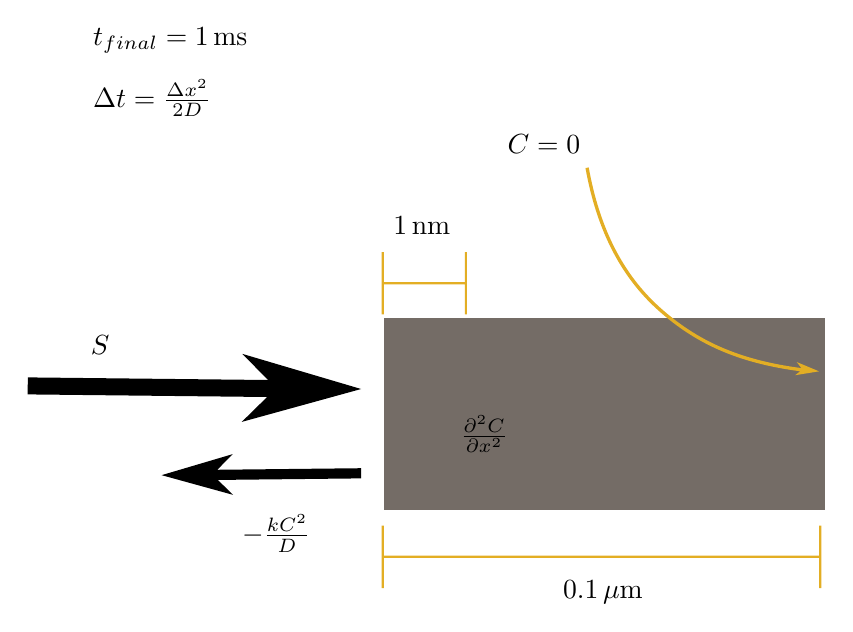
\begin{tikzpicture}[y=0.80pt, x=0.8pt,yscale=-1, inner sep=0pt, outer sep=0pt]
\begin{scope}[shift={(0,-579.86215)}]
  \path[fill=c746c66,line join=miter,line cap=butt,even odd rule,line
    width=1.327pt] (200.9106,774.0675) -- (400.0000,774.0675) --
    (400.0000,860.6569) -- (200.9106,860.6569) -- cycle;
  \path[color=black,fill=black,line join=miter,line cap=butt,miter limit=4.00,even
    odd rule,line width=2.400pt] (136.8727,790.1525) -- (190.5000,806.0161) --
    (136.5876,820.8745) -- (148.0503,809.6270) -- (39.8955,808.4517) --
    (39.9554,800.7699) -- (148.4553,801.9502) -- (136.8726,790.1525) -- cycle;
  \path[fill=black,line join=miter,line cap=butt,line width=0.800pt]
    (68.41143,790.55756) node[above right] (text4542) {$S$};
  \path[fill=black,line join=miter,line cap=butt,line width=0.800pt]
    (235.29883,834.88702) node[above right] (text4986) {$\frac{\partial^{2}
    C}{\partial x^{2}}$};
  \path[color=black,fill=black,line join=miter,line cap=butt,miter limit=4.00,even
    odd rule,line width=2.400pt] (132.4778,835.4371) -- (100.3922,844.9285) --
    (132.6483,853.8184) -- (125.7902,847.0889) -- (190.5000,846.3857) --
    (190.4642,841.7896) -- (125.5479,842.4958) -- (132.4779,835.4371) -- cycle;
  \path[fill=black,line join=miter,line cap=butt,line width=0.800pt]
    (136.73097,879.73804) node[above right] (text5169) {$-\frac{kC^{2}}{D}$};
  \path[fill=black,line join=miter,line cap=butt,line width=0.800pt]
    (256.6813,699.8125) node[above right] (text5222) {$C=0$};
  \path[shift={(0,579.86215)},color=black,fill=ce3ae24,line join=miter,line
    cap=butt,miter limit=4.00,even odd rule,line width=1.200pt]
    (293.3125,126.0762) -- (291.8359,126.3418) .. controls (296.8118,154.0147) and
    (307.5794,175.3619) .. (324.7363,190.6562) .. controls (341.3228,205.4422) and
    (360.1433,214.3391) .. (388.7988,218.1465) -- (386.5469,219.9238) --
    (397.3262,218.1719) -- (387.2480,213.9648) -- (389.4199,216.7148) .. controls
    (360.7321,212.9672) and (342.1269,204.1501) .. (325.7344,189.5371) .. controls
    (308.8619,174.4962) and (298.2455,153.5109) .. (293.3125,126.0762) -- cycle;
  \path[color=black,fill=ce3ae24,line join=miter,line cap=butt,miter
    limit=4.00,even odd rule,line width=0.800pt] (199.7656,867.7438) --
    (199.7656,881.3239) -- (199.7441,881.3239) -- (199.7441,882.3239) --
    (199.7656,882.3239) -- (199.7656,895.9059) -- (200.7656,895.9059) --
    (200.7656,882.3239) -- (397.4219,882.3239) -- (397.4219,895.9059) --
    (398.4219,895.9059) -- (398.4219,867.7438) -- (397.4219,867.7438) --
    (397.4219,881.3239) -- (200.7656,881.3239) -- (200.7656,867.7438) --
    (199.7656,867.7438) -- cycle;
  \path[fill=black,line join=miter,line cap=butt,line width=0.800pt]
    (281.71442,903.20654) node[above right] (text5330) {$0.1\,\mathrm{\mu m}$};
  \path[color=black,fill=ce3ae24,line join=miter,line cap=butt,miter
    limit=4.00,even odd rule,line width=0.800pt] (199.7656,744.1422) --
    (199.7656,757.7222) -- (199.7441,757.7222) -- (199.7441,758.7222) --
    (199.7656,758.7222) -- (199.7656,772.3043) -- (200.7656,772.3043) --
    (200.7656,758.7222) -- (237.3145,758.7222) -- (237.3145,772.3043) --
    (238.3145,772.3043) -- (238.3145,744.1422) -- (237.3145,744.1422) --
    (237.3145,757.7222) -- (200.7656,757.7222) -- (200.7656,744.1422) --
    (199.7656,744.1422) -- cycle;
  \path[fill=black,line join=miter,line cap=butt,line width=0.800pt]
    (205.05051,736.31909) node[above right] (text5347) {$1\,\mathrm{nm}$};
  \path[fill=black,line join=miter,line cap=butt,line width=0.800pt]
    (69.454475,654.44) node[above right] (text5355) {$t_{final}=1\,\mathrm{ms}$};
  \path[fill=black,line join=miter,line cap=butt,line width=0.800pt]
    (69.454475,683.12378) node[above right] (text5359) {$\Delta t = \frac{\Delta
    x^{2}}{2D}$};
\end{scope}

\end{tikzpicture}
